% Created by tikzDevice version 0.8.1 on 2015-02-22 23:55:08
% !TEX encoding = UTF-8 Unicode
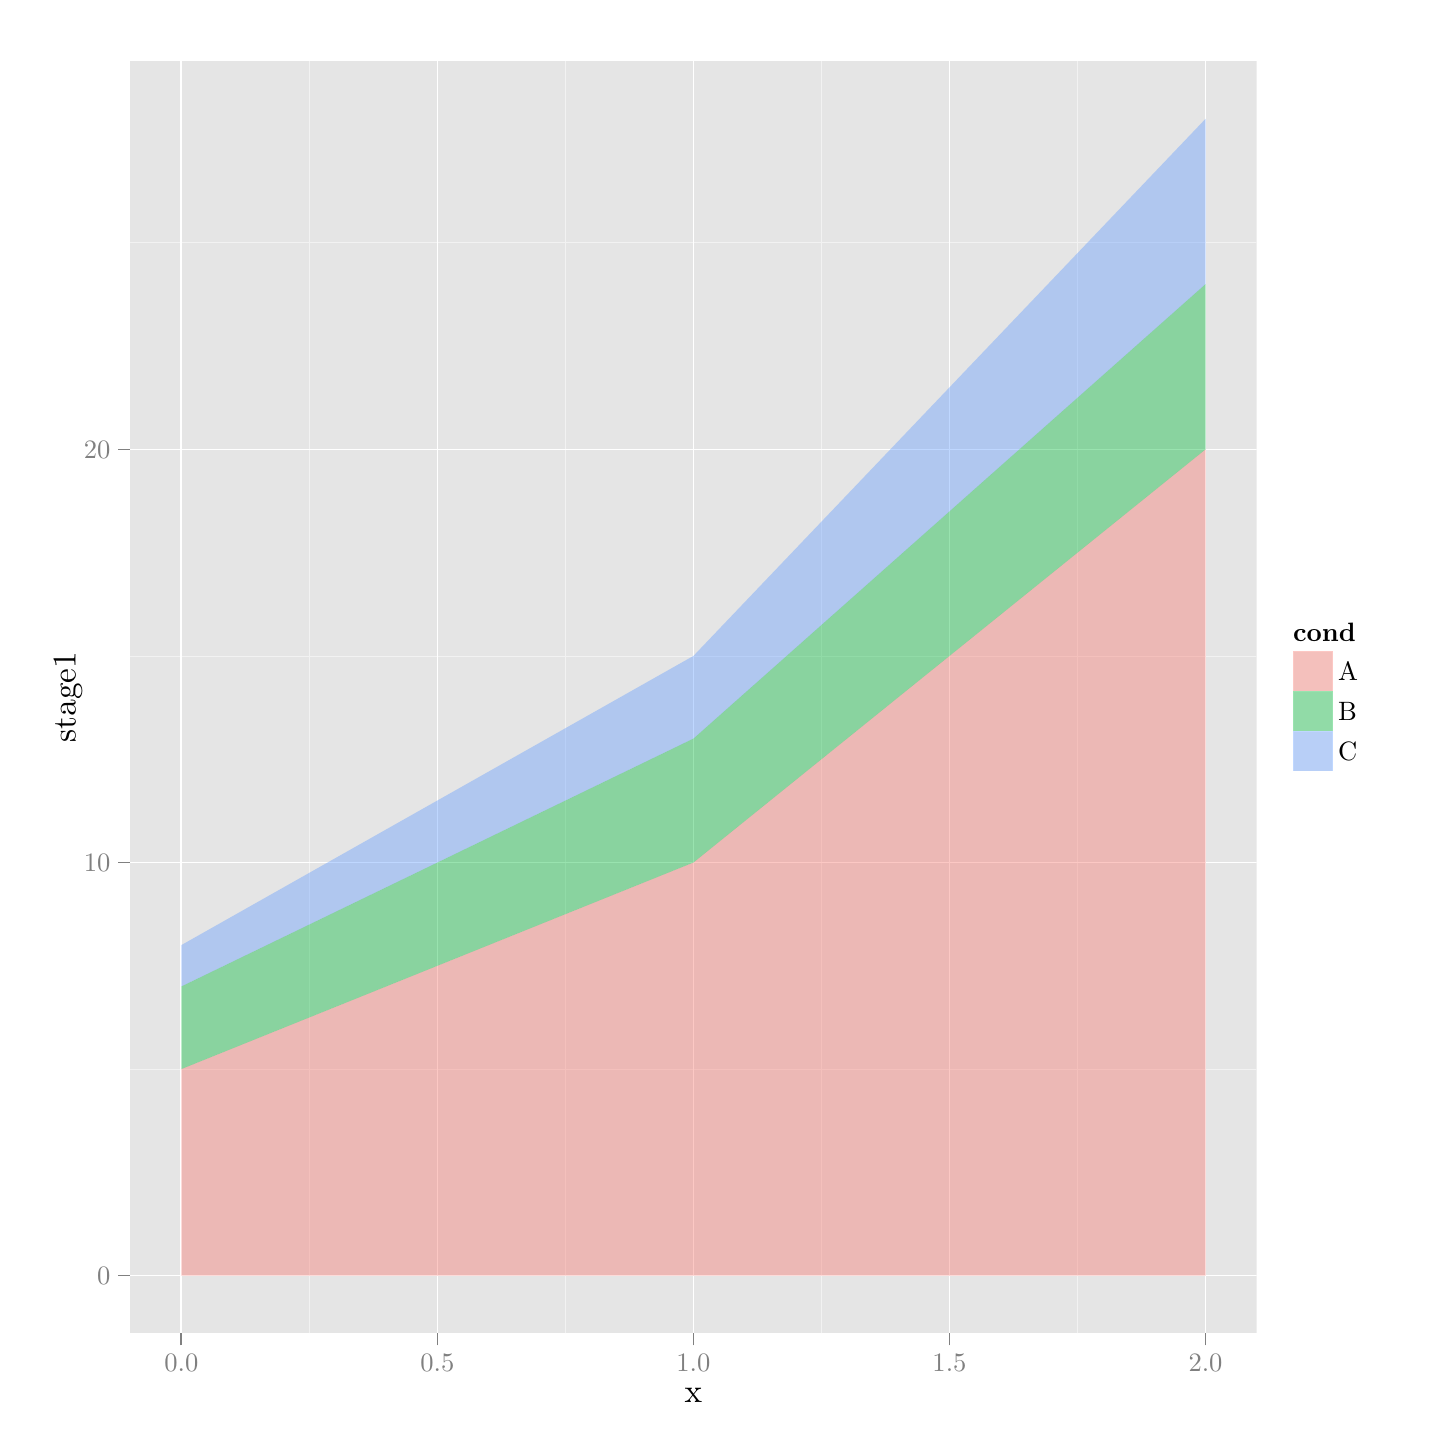
\begin{tikzpicture}[x=1pt,y=1pt]
\definecolor{fillColor}{RGB}{255,255,255}
\path[use as bounding box,fill=fillColor,fill opacity=0.00] (0,0) rectangle (505.89,505.89);
\begin{scope}
\path[clip] (  0.00,  0.00) rectangle (505.89,505.89);
\definecolor{drawColor}{RGB}{255,255,255}
\definecolor{fillColor}{RGB}{255,255,255}

\path[draw=drawColor,line width= 0.6pt,line join=round,line cap=round,fill=fillColor] (  0.00,  0.00) rectangle (505.89,505.89);
\end{scope}
\begin{scope}
\path[clip] ( 37.02, 34.03) rectangle (444.11,493.85);
\definecolor{fillColor}{gray}{0.90}

\path[fill=fillColor] ( 37.02, 34.03) rectangle (444.11,493.85);
\definecolor{drawColor}{gray}{0.95}

\path[draw=drawColor,line width= 0.3pt,line join=round] ( 37.02,129.58) --
	(444.11,129.58);

\path[draw=drawColor,line width= 0.3pt,line join=round] ( 37.02,278.87) --
	(444.11,278.87);

\path[draw=drawColor,line width= 0.3pt,line join=round] ( 37.02,428.16) --
	(444.11,428.16);

\path[draw=drawColor,line width= 0.3pt,line join=round] (101.79, 34.03) --
	(101.79,493.85);

\path[draw=drawColor,line width= 0.3pt,line join=round] (194.31, 34.03) --
	(194.31,493.85);

\path[draw=drawColor,line width= 0.3pt,line join=round] (286.83, 34.03) --
	(286.83,493.85);

\path[draw=drawColor,line width= 0.3pt,line join=round] (379.35, 34.03) --
	(379.35,493.85);
\definecolor{drawColor}{RGB}{255,255,255}

\path[draw=drawColor,line width= 0.6pt,line join=round] ( 37.02, 54.94) --
	(444.11, 54.94);

\path[draw=drawColor,line width= 0.6pt,line join=round] ( 37.02,204.22) --
	(444.11,204.22);

\path[draw=drawColor,line width= 0.6pt,line join=round] ( 37.02,353.51) --
	(444.11,353.51);

\path[draw=drawColor,line width= 0.6pt,line join=round] ( 55.52, 34.03) --
	( 55.52,493.85);

\path[draw=drawColor,line width= 0.6pt,line join=round] (148.05, 34.03) --
	(148.05,493.85);

\path[draw=drawColor,line width= 0.6pt,line join=round] (240.57, 34.03) --
	(240.57,493.85);

\path[draw=drawColor,line width= 0.6pt,line join=round] (333.09, 34.03) --
	(333.09,493.85);

\path[draw=drawColor,line width= 0.6pt,line join=round] (425.61, 34.03) --
	(425.61,493.85);
\definecolor{fillColor}{RGB}{248,118,109}

\path[fill=fillColor,fill opacity=0.40] ( 55.52,129.58) --
	(240.57,204.22) --
	(425.61,353.51) --
	(425.61, 54.94) --
	(240.57, 54.94) --
	( 55.52, 54.94) --
	cycle;
\definecolor{fillColor}{RGB}{0,186,56}

\path[fill=fillColor,fill opacity=0.40] ( 55.52,159.44) --
	(240.57,249.01) --
	(425.61,413.23) --
	(425.61,353.51) --
	(240.57,204.22) --
	( 55.52,129.58) --
	cycle;
\definecolor{fillColor}{RGB}{97,156,255}

\path[fill=fillColor,fill opacity=0.40] ( 55.52,174.37) --
	(240.57,278.87) --
	(425.61,472.94) --
	(425.61,413.23) --
	(240.57,249.01) --
	( 55.52,159.44) --
	cycle;
\end{scope}
\begin{scope}
\path[clip] (  0.00,  0.00) rectangle (505.89,505.89);
\definecolor{drawColor}{gray}{0.50}

\node[text=drawColor,anchor=base east,inner sep=0pt, outer sep=0pt, scale=  0.96] at ( 29.91, 51.63) {0};

\node[text=drawColor,anchor=base east,inner sep=0pt, outer sep=0pt, scale=  0.96] at ( 29.91,200.92) {10};

\node[text=drawColor,anchor=base east,inner sep=0pt, outer sep=0pt, scale=  0.96] at ( 29.91,350.21) {20};
\end{scope}
\begin{scope}
\path[clip] (  0.00,  0.00) rectangle (505.89,505.89);
\definecolor{drawColor}{gray}{0.50}

\path[draw=drawColor,line width= 0.6pt,line join=round] ( 32.75, 54.94) --
	( 37.02, 54.94);

\path[draw=drawColor,line width= 0.6pt,line join=round] ( 32.75,204.22) --
	( 37.02,204.22);

\path[draw=drawColor,line width= 0.6pt,line join=round] ( 32.75,353.51) --
	( 37.02,353.51);
\end{scope}
\begin{scope}
\path[clip] (  0.00,  0.00) rectangle (505.89,505.89);
\definecolor{drawColor}{gray}{0.50}

\path[draw=drawColor,line width= 0.6pt,line join=round] ( 55.52, 29.77) --
	( 55.52, 34.03);

\path[draw=drawColor,line width= 0.6pt,line join=round] (148.05, 29.77) --
	(148.05, 34.03);

\path[draw=drawColor,line width= 0.6pt,line join=round] (240.57, 29.77) --
	(240.57, 34.03);

\path[draw=drawColor,line width= 0.6pt,line join=round] (333.09, 29.77) --
	(333.09, 34.03);

\path[draw=drawColor,line width= 0.6pt,line join=round] (425.61, 29.77) --
	(425.61, 34.03);
\end{scope}
\begin{scope}
\path[clip] (  0.00,  0.00) rectangle (505.89,505.89);
\definecolor{drawColor}{gray}{0.50}

\node[text=drawColor,anchor=base,inner sep=0pt, outer sep=0pt, scale=  0.96] at ( 55.52, 20.31) {0.0};

\node[text=drawColor,anchor=base,inner sep=0pt, outer sep=0pt, scale=  0.96] at (148.05, 20.31) {0.5};

\node[text=drawColor,anchor=base,inner sep=0pt, outer sep=0pt, scale=  0.96] at (240.57, 20.31) {1.0};

\node[text=drawColor,anchor=base,inner sep=0pt, outer sep=0pt, scale=  0.96] at (333.09, 20.31) {1.5};

\node[text=drawColor,anchor=base,inner sep=0pt, outer sep=0pt, scale=  0.96] at (425.61, 20.31) {2.0};
\end{scope}
\begin{scope}
\path[clip] (  0.00,  0.00) rectangle (505.89,505.89);
\definecolor{drawColor}{RGB}{0,0,0}

\node[text=drawColor,anchor=base,inner sep=0pt, outer sep=0pt, scale=  1.20] at (240.57,  9.03) {x};
\end{scope}
\begin{scope}
\path[clip] (  0.00,  0.00) rectangle (505.89,505.89);
\definecolor{drawColor}{RGB}{0,0,0}

\node[text=drawColor,rotate= 90.00,anchor=base,inner sep=0pt, outer sep=0pt, scale=  1.20] at ( 17.30,263.94) {stage1};
\end{scope}
\begin{scope}
\path[clip] (  0.00,  0.00) rectangle (505.89,505.89);
\definecolor{fillColor}{RGB}{255,255,255}

\path[fill=fillColor] (452.98,232.87) rectangle (484.98,295.01);
\end{scope}
\begin{scope}
\path[clip] (  0.00,  0.00) rectangle (505.89,505.89);
\definecolor{drawColor}{RGB}{0,0,0}

\node[text=drawColor,anchor=base west,inner sep=0pt, outer sep=0pt, scale=  0.96] at (457.25,284.11) {\bfseries cond};
\end{scope}
\begin{scope}
\path[clip] (  0.00,  0.00) rectangle (505.89,505.89);
\definecolor{drawColor}{RGB}{255,255,255}
\definecolor{fillColor}{gray}{0.95}

\path[draw=drawColor,line width= 0.6pt,line join=round,line cap=round,fill=fillColor] (457.25,266.05) rectangle (471.70,280.50);
\end{scope}
\begin{scope}
\path[clip] (  0.00,  0.00) rectangle (505.89,505.89);
\definecolor{fillColor}{RGB}{248,118,109}

\path[fill=fillColor,fill opacity=0.40] (457.25,266.05) rectangle (471.70,280.50);

\path[] (457.25,266.05) --
	(471.70,280.50);
\end{scope}
\begin{scope}
\path[clip] (  0.00,  0.00) rectangle (505.89,505.89);
\definecolor{drawColor}{RGB}{255,255,255}
\definecolor{fillColor}{gray}{0.95}

\path[draw=drawColor,line width= 0.6pt,line join=round,line cap=round,fill=fillColor] (457.25,251.59) rectangle (471.70,266.05);
\end{scope}
\begin{scope}
\path[clip] (  0.00,  0.00) rectangle (505.89,505.89);
\definecolor{fillColor}{RGB}{0,186,56}

\path[fill=fillColor,fill opacity=0.40] (457.25,251.59) rectangle (471.70,266.05);

\path[] (457.25,251.59) --
	(471.70,266.05);
\end{scope}
\begin{scope}
\path[clip] (  0.00,  0.00) rectangle (505.89,505.89);
\definecolor{drawColor}{RGB}{255,255,255}
\definecolor{fillColor}{gray}{0.95}

\path[draw=drawColor,line width= 0.6pt,line join=round,line cap=round,fill=fillColor] (457.25,237.14) rectangle (471.70,251.59);
\end{scope}
\begin{scope}
\path[clip] (  0.00,  0.00) rectangle (505.89,505.89);
\definecolor{fillColor}{RGB}{97,156,255}

\path[fill=fillColor,fill opacity=0.40] (457.25,237.14) rectangle (471.70,251.59);

\path[] (457.25,237.14) --
	(471.70,251.59);
\end{scope}
\begin{scope}
\path[clip] (  0.00,  0.00) rectangle (505.89,505.89);
\definecolor{drawColor}{RGB}{0,0,0}

\node[text=drawColor,anchor=base west,inner sep=0pt, outer sep=0pt, scale=  0.96] at (473.51,269.97) {A};
\end{scope}
\begin{scope}
\path[clip] (  0.00,  0.00) rectangle (505.89,505.89);
\definecolor{drawColor}{RGB}{0,0,0}

\node[text=drawColor,anchor=base west,inner sep=0pt, outer sep=0pt, scale=  0.96] at (473.51,255.51) {B};
\end{scope}
\begin{scope}
\path[clip] (  0.00,  0.00) rectangle (505.89,505.89);
\definecolor{drawColor}{RGB}{0,0,0}

\node[text=drawColor,anchor=base west,inner sep=0pt, outer sep=0pt, scale=  0.96] at (473.51,241.06) {C};
\end{scope}
\end{tikzpicture}
